\documentclass[UTF8]{ctexart}

\usepackage{WeeklyReport}
\usepackage{graphicx}
\usepackage{amsmath}
\usepackage{amssymb}

\title{周报05}
\author{Jeff\ Fu}
\date{\today}

\begin{document}
    \maketitle
    % \tableofcontents
    \section{本周计划}
        \begin{itemize}
            \item 阅读相关论文,整理思路
        \end{itemize}
    \section{收获}
        这周看了Teacher Student Model和Mutual Learning方面的文章,
        整理了一下文章中值得借鉴的想法
        \subsection{Teacher Student Model}
            \subsubsection{基本思路}
                Teacher Student Model的模型包含两个部分,
                Teacher和Student,用Teacher去引导Student学习知识(知识蒸馏?)

                在半监督学习的过程中,将unlabeled data作为regularization

                Consistency Regularization:同一组input,经过不同的Data Augmentation和Dropout,
                model能得到一致的结果(经softmax后得到的soft label)
            \subsubsection{Temporal Ensembling for Semi-Supervised Learning}
                如图 \ref{fig:TE} 所示,文章提出了两个model。
                \begin{figure}[ht]
                    \centering
                    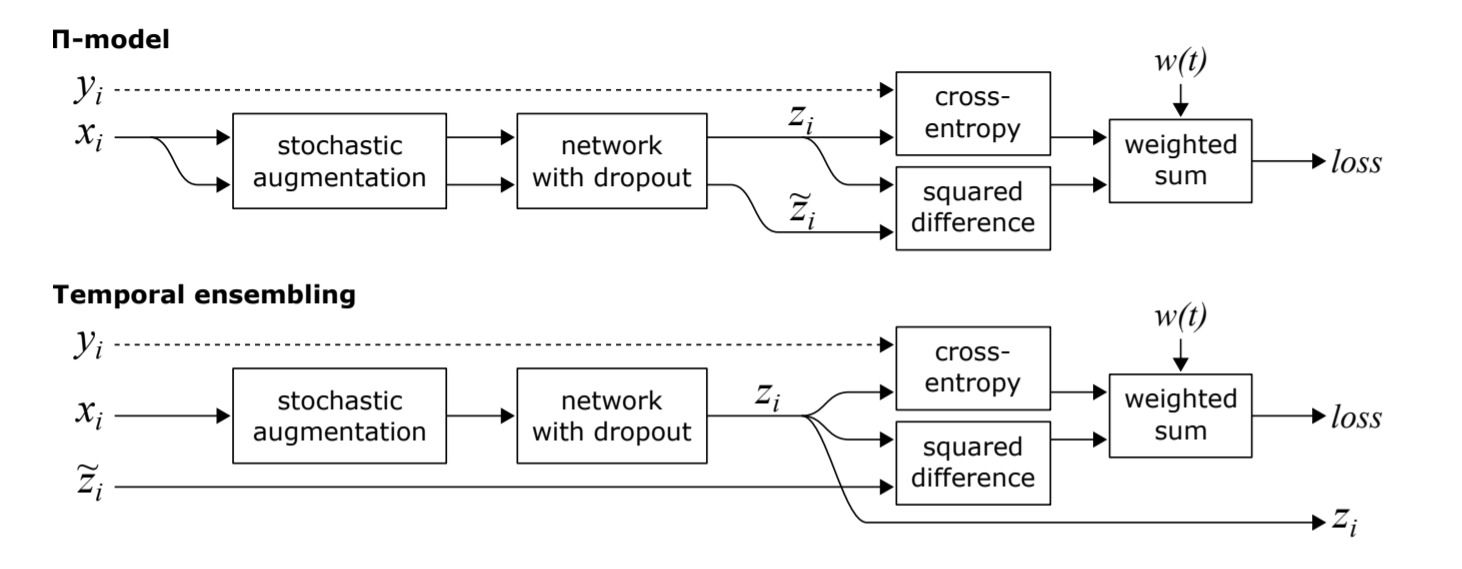
\includegraphics[scale=0.34]{Week05_Temporal_Ensembling.png}
                    \caption{$\Pi$-model和Temporal Ensembling}
                    \label{fig:TE}
                \end{figure}

                \textbf{$\Pi$-model}

                teacher和student分别通过不同的数据增强(文中使用的是noise)和dropout,
                在teacher和student之间设计consistency loss(teacher和student的选择是任意的吗?图示中只有student参与了cross entropy的计算)

                在训练的初期,consistency loss的权重为0(此时teacher的结果还不可靠,先使用cross entropy loss进行supervised learning)
                ,随着epoch增加,consistency loss的权重越来越大

                \textbf{Temporal Ensembling}

                teacher的输出可能是不可靠的,通过ensemble去解决,
                即将最近几个epoch的预测结果进行ensemble得到新的预测(相当于是从student的输出得到teacher?):

                $$
                    Z_i \leftarrow \alpha Z_i + (1-\alpha)z_i
                $$

                $$
                    \tilde{z}_i \leftarrow \frac{Z_i}{1-{\alpha}^t}
                $$

                其中 $t$ 表示第 $t$ 个epoch。
            \subsubsection{Mean teachers are better role models: Weight-averaged consistency targets improve semi-supervised deep learning results}
                前面的temporal ensemble也存在缺陷,当label信息比较多时,空间开销较大,并且 $\tilde{z}$ 的更新具有滞后性(一个epoch更新一次)。
                为了解决这些问题,提出了如图 \ref{fig:MT} 所示的Mean Teacher方法。

                在Mean Teacher方法中,teacher和student都对input进行预测,只是使用不同的noise,
                student得到的结果分别于label(cross entropy)和teacher(consistency)计算loss。
                在更新参数时,先更新student,teacher的参数再通过指数级流动平均
                (exponential moving average,即指数级的累计平均值)得到。
                \begin{figure}[ht]
                    \centering
                    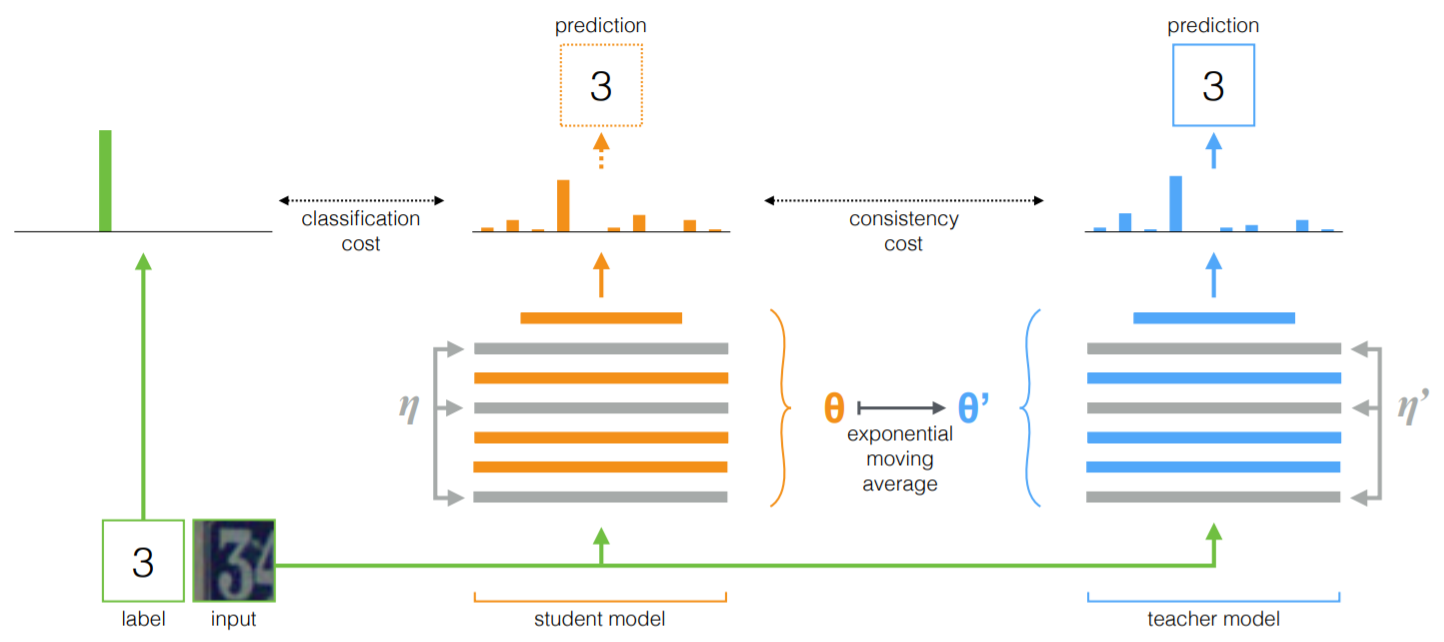
\includegraphics[scale=0.34]{Week05_Mean_Teacher.png}
                    \caption{Mean Teacher方法}
                    \label{fig:MT}
                \end{figure}
            \subsubsection{Teacher Student小结(半监督学习)}
                在Teacher Student模型中,Teacher和Student使用不同的数据增强和dropout,
                student可以与带label的数据构成cross entropy,teacher的输出最终与student的输出计算consistency loss,
                Teacher 与 Student使用不同的数据增强(也可以是扰动,如noise)和dropout,但要求teacher和student的输出是一致的。

                Teacher Student Model有效的原因:

                \begin{enumerate}
                    \item 在半监督学习中,假设不同类别的分界线处数据的分布是低密度的(随机扰动不会改变label,而随机扰动使得模型不易over fit)
                    \item 一致性loss使得模型具有更好的鲁棒性(在feature space上趋于一致,多个高维数据点被映射到临近的低维数据点)
                \end{enumerate}
        \subsection{Deep Mutual Learning}
            \subsubsection{Motivation}
                深度神经网络的参数量太大,需要庞大的计算量,这篇文章考虑对深度网络进行模型蒸馏(知识传递)。

                传统的模型蒸馏算法需要预先训练一个大网络,把大网络当作teacher向小网络传递知识,
                从而提高小网络的性能。而Deep Mutual Learning的想法则是让小网络之间互相学习共同进步。
            \subsubsection{方法}
                多个网络同时进行训练,引入两种loss,一个是常规的分类loss(如cross entropy),另一个是不同网络之间的交互损失。

                使用交叉熵和KL散度衡量监督学习的loss和互学习的loss(假设进行两个网络的mutual learning):

                $$
                    p_{1}^{m}(\boldsymbol{x}_i) = \frac{exp(z_{1}^{m})}{\sum_{m=1}^{M} exp(z_{1}^{m})}
                $$

                $$
                    L_{C_{1}} = - \sum_{i=1}^{N} \sum_{m=1}^{M} I(y_{i}, m) \log(p_{1}^{m}(\boldsymbol{x}_i))
                $$

                $$
                    D_{KL}(\boldsymbol{p}_{2}\|\boldsymbol{p}_{1}) = \sum_{i=1}^{N} \sum_{m=1}^{M} p_{2}^{m}(\boldsymbol{x}_i) \log \frac{p_{2}^{m}(\boldsymbol{x}_i)}{p_{1}^{m}(\boldsymbol{x}_i)}
                $$

                于是第一个网络的Loss可以写成:

                $$
                    L_{\Theta_{1}} = L_{C_{1}} + D_{KL}(\boldsymbol{p}_{2}\|\boldsymbol{p}_{1})
                $$

                同理,第二个网络的Loss可以写成:

                $$
                    L_{\Theta_{2}} = L_{C_{2}} + D_{KL}(\boldsymbol{p}_{1}\|\boldsymbol{p}_{2})
                $$

                在训练的时候,交替迭代更新两个网络的参数。
    \section{启发}
        \begin{enumerate}
            \item 如果把Teacher Student Model应用到NPN中,将未添加NPN的网络作为Teacher,
                添加了NPN的网络作为Student,在两者之间可以设计Consistency Loss,训练完成后,
                测试时把Student的NPN去掉,也许能获得更好的结果(如果把NPN放在Feature Extractor上,
                相当于是把Feature Map模糊化,如果放在Classifier上,
                相当于是给Classifier增大了分类难度)
            \item 感觉上NPN可以换成noise,甚至也可以换成Teacher Student Model中的Data Augmentation
            \item NPN的优化过程可以联想到极大极小值搜索和alpha-beta剪枝等传统算法(不确定)
            \item 如果把Mutual Learning的想法应用到Multi-Source DA上,可以给每个source分别安排一个网络,
                由这些网络共同向一个中心网络传递知识,然后这个中心网络再将知识进行提炼得到multi-source的效果。
                或者直接照搬Deep Mutual Learning,使用两个多源的网络进行相互训练。
            \item (这个想法是从“蒸馏”这个词想到的,跟论文好像没什么联系)前面提到模型蒸馏算法是为了提高性能,
                而原始的模型蒸馏指的是用大网络辅助训练小网络。我的想法是,能否让网络在训练的过程中,
                自主“退化”掉一些不必要的神经元(实际情况下指的是权重参数为0,但每一层的神经元数是固定的,所以那些神经元仍然在占用运算资源),
                反过来想,是否也可以自主“进化”(同样因为每一层的维数是固定的,这个想法可能只是空想)
        \end{enumerate}
    \section{疑问/困难}
        \begin{enumerate}
            \item 之前的PAL是直接在原模型的基础上添加的,如果要采用新的思路(Teacher Student或Mutual Learning),
                可能需要把原来的模型结构和Loss抛弃(如k-moment)
            \item 现在反过来想,之前引入PAL其实使得网络更复杂了,结果的提升可能主要原因在于网络参数变多而不是PAL本身,
                详细情况等做了DomainNet的实验后再确定
        \end{enumerate}
\end{document}
